% Generated by Sphinx.
\def\sphinxdocclass[english]{xmosmodern}
\documentclass[  collection]{xmosmodern}
\usepackage[utf8]{inputenc}
\DeclareUnicodeCharacter{00A0}{\nobreakspace}

\usepackage{longtable}



\title{A16 sliceKIT Hardware Manual}
\date{March 19, 2014}
\author{}
\newcommand{\sphinxlogo}{}
\newcommand{\releasename}{Release}
\usepackage{xsphinx}
\usepackage{threeparttable}
\usepackage{fancyvrb}
\usepackage{indent}
\renewcommand\bfcode\textbf
\renewcommand\bf\textbf
\graphicspath{{./}{./images/}}
\makeindex

\newcommand\PYGZat{@}
\newcommand\PYGZlb{[}
\newcommand\PYGZrb{]}

\setlength{\emergencystretch}{8em}
\start

\maketitle
\pretoc
\phantomsection\label{index::doc}

%summary!

% NON-FULLWIDTH SECTION



% NON-FULLWIDTH SECTION
\clearpage
\chapter{Overview}
\label{overview:a16-slicekit-overview}\label{overview:a16-slicekit-hardware-manual}\label{overview::doc}%summary!
\begin{inthisdocument}
\item \nameref{overview:introduction}
\item \nameref{overview:slicekit-system-layout}
\end{inthisdocument}




% NON-FULLWIDTH SECTION
\section{Introduction}
\label{overview:introduction}

This document covers the hardware design of the sliceKIT Modular Development System, consisting of the A16 Core Board, sliceCARDs and XSYS adaptor.


The Core Board contains a fully pinned out 16-core xCORE Processor, with its GPIOs connected to four expansion connectors (termed \verb`Slots`) to interface with expansion cards called sliceCARDs which plug into the slots. The Core Board also contains all circuitry necessary for operating and debugging the XMOS system. Multiple sliceKIT Core Boards can be interconnected to form a multi XMOS device system with dual 5-bit xCONNECT Links being present between the boards.


\newpage



% NON-FULLWIDTH SECTION
\section{sliceKIT system layout}
\label{overview:slicekit-system-layout}\begin{figure}[h]
\begin{sidecaption}{sliceKIT Layout}

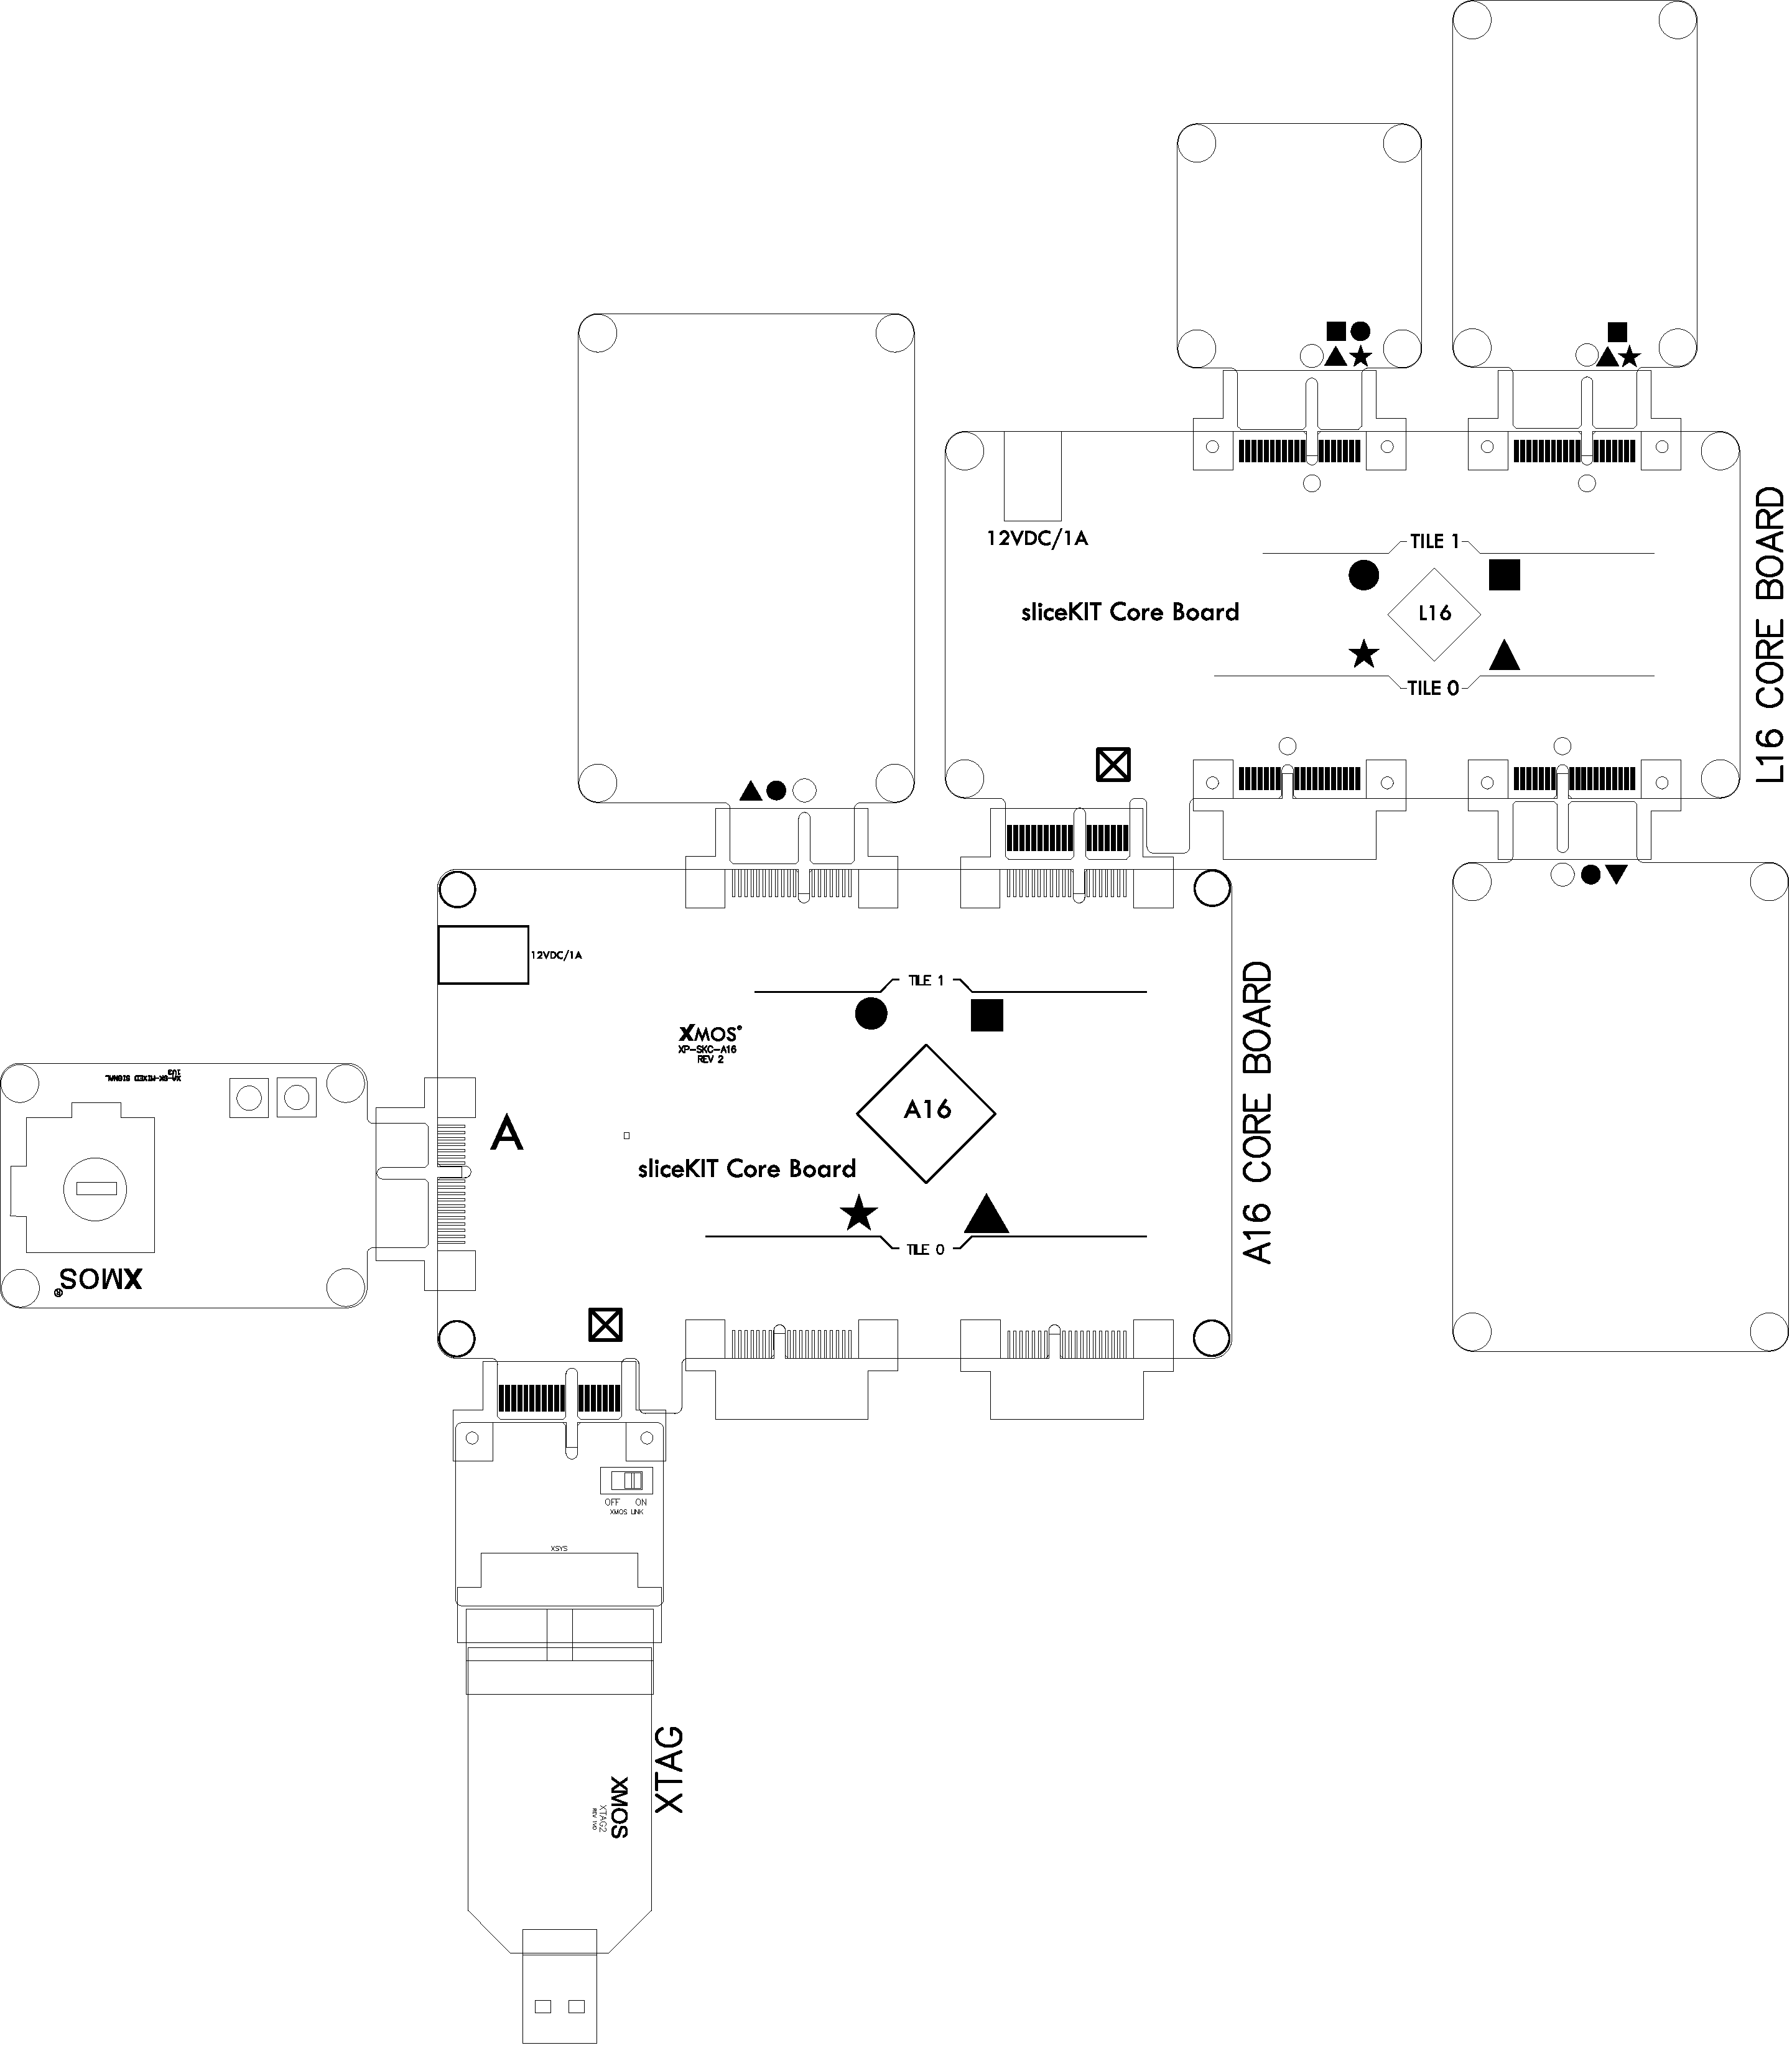
\includegraphics[width=1.000\linewidth]{slicekitlayout.pdf}
\end{sidecaption}\end{figure} \DocumentFooterFix


The diagram above shows an overview of the layout of the core board with slice boards attached. Each of the four slots has a specific label - \verb`Star`, \verb`Triangle`, \verb`Square` and \verb`Circle`, printed on the Core Board silkscreen.  \verb`Triangle` and \verb`Circle` sliceCARDs contain 24 xCORE I/Os and \verb`Star` and \verb`Square` sliceCARDs 20 xCORE I/Os (usable as GPIO or two 5-wire XMOS links). The label denotes which sliceCARDs are compatible with which Core Board Slots. The sliceCARDs are also marked with one or more of these labels to identify the slot type(s) they function correctly with.


In addition to the four standard sliceCARD slots there is a \verb`Mixed Signal` slot, labelled A, this slot has access to the 8 ADC channels available on the A16 device, along with 4 xCORE I/Os and the wake pin. The xCORE I/Os available on the \verb`Mixed Signal` slot overlap with the \verb`Star` slot, meaning that if the \verb`Mixed Signal` I/Os are used then a sliceCARD used in the \verb`Star` slot may not function.


The final type of connector is on the bottom left of the Core Board and is marked with a hollow square symbol with an X through it. This is for connecting multiple Core Boards together to form systems of 32 logical cores or more. It is termed the \verb`chain` slot.


All Slots are 36 pin PCI express style connectors in either socket or edge finger (plug) types.


\verb`Star`, \verb`Triangle` and \verb`Mixed Signal` Slots are pinned out from Tile 0 of the A16 xCORE and the \verb`Circle` and \verb`Square` Slots from Tile 1.



% NON-FULLWIDTH SECTION
\clearpage
\chapter{Core Board}
\label{a16_core_board:a16-slicekit-core-board}\label{a16_core_board::doc}%summary!
\begin{inthisdocument}
\item \nameref{a16_core_board:multiple-core-boards}
\item \nameref{a16_core_board:setup}
\item \nameref{a16_core_board:power-supply}
\item \nameref{a16_core_board:debug}
\item \nameref{a16_core_board:a16-boot}
\item \nameref{a16_core_board:xconnect-links}
\item \nameref{a16_core_board:reset}
\item \nameref{a16_core_board:clocking}
\item \nameref{a16_core_board:testpoints}
\item \nameref{a16_core_board:slot-pinouts}
\end{inthisdocument}



This board contains the XMOS device plus support circuitry.


A single XS1-A16A-128 device has all of its GPIO connected to the Slots.
\begin{figure}[h]
\begin{sidecaption}{A16 sliceKIT Core Board}

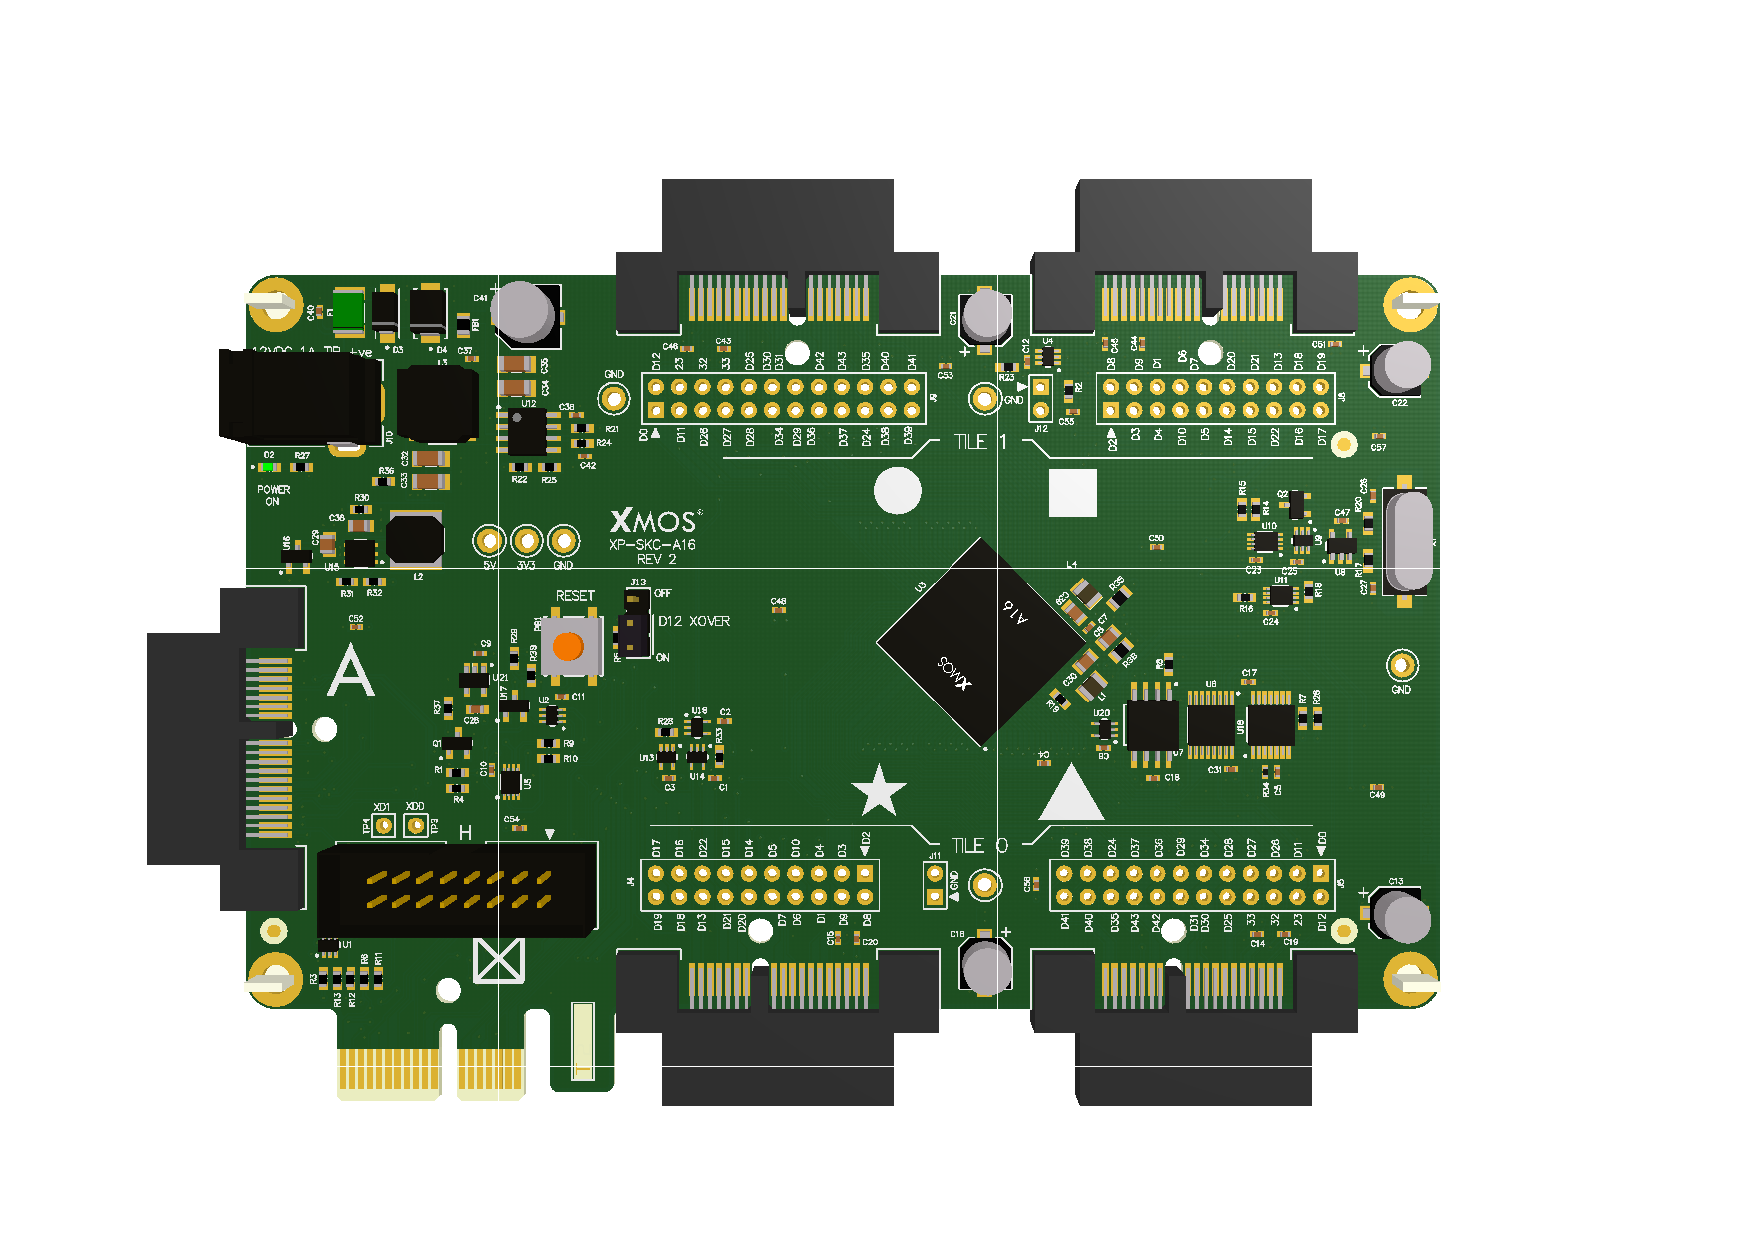
\includegraphics[width=0.900\linewidth]{a16_core_board.pdf}
\end{sidecaption}\end{figure} \DocumentFooterFix



% NON-FULLWIDTH SECTION
\section{Multiple Core Boards}
\label{a16_core_board:multiple-core-boards}

Additional A16 or L16 sliceKIT Core Boards can be connected to the first board's \verb`Chain` slot via the second board's \verb`Square` Slot to add extra processing capability and I/O through extra Slice Cards. The first such board is termed the Master, the remaining boards as Slaves. When there is only one board, it is the Master.



% NON-FULLWIDTH SECTION
\section{Setup}
\label{a16_core_board:setup}

For debugging, an XSYS adaptor board is connected to the \verb`Chain` Connector of the Master Board to allow connection of an xTAG debug adapter to provide a debug link from a USB host.


The Core Board is powered by a 12V external power supply.



% NON-FULLWIDTH SECTION
\section{Power Supply}
\label{a16_core_board:power-supply}

Power input to the sliceKIT Core Board is via a standard barrel jack connector. A standard 12V external power supply should be used to power the board. Each Core Board requires its own 12V supply. This input supply is used to generate the main 5V board supply via a DC-DC converter.


The 5V board supply is then fed to all the Slot connectors as well as powering the Core Board itself. A 3V3 supply is generated by DC-DC converters from the 5V main supply.


The A16 device uses integrated DC-DC converters to generate the 1V8 and 1V0 supplies required by the device.


The supplies are sequenced to ensure the power up sequence is 5V then 3V3. When the 3V3 supply is good then the system will be released from reset.


The Core Board provides 3V3 and 5V at 0.25A each for a total of approximately 2W per slice.



% NON-FULLWIDTH SECTION
\section{Debug}
\label{a16_core_board:debug}

Debug of the system is via the XSYS adapter board connected to the \verb`Chain` Connector.


The JTAG signals are connected as shown below.
\begin{figure}[h]
\begin{sidecaption}{JTAG Chain}

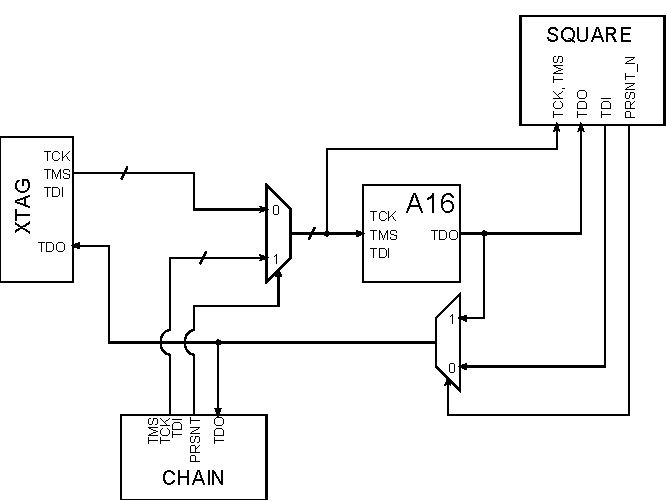
\includegraphics[width=0.700\linewidth]{jtagchain.pdf}
\end{sidecaption}\end{figure} \DocumentFooterFix


Presence detect signals are present on both the \verb`Chain` Connector and \verb`Square` Slot connectors to allow detection of a connected board and subsequent automatic switching of the JTAG chain.  In a system of multiple Core Boards, the Master is the source of the JTAG chain so the system can only be debugged from the master. Other boards will see no devices in the JTAG chain.


The use of xSCOPE is covered in the xCONNECT Links section. The xSCOPE xCONNECT link can be either enabled or disabled via a switch on the XSYS adapter board.



% NON-FULLWIDTH SECTION
\section{A16 Boot}
\label{a16_core_board:a16-boot}

Master Core Boards boot from SPI flash, while slave Core Boards boot from xCONNECT link \verb`XLB` from the next connected Core Board.


To allow re-use of the SPI boot pins (ports 1A, 1B, 1C, 1D) as signal I/O pins for the \verb`Star`, \verb`Triangle` and \verb`A` slot, a latched bus switch is used which connects the xCORE SPI pins to either the SPI Flash or to the Slice Card Slots. The switch is controlled by X0D42 and X0D43 (P8D6 and P8D7 on Tile 0: on the \verb`Triangle` slot). Once the device has booted X0D43 is used to enable or disable the SPI interface, X0D42 should then transition from low to high to latch the selection. The SPI selection state is then maintained until the system is reset.
\begin{figure}[h]
\begin{sidecaption}{SPI Select Flow Diagram}

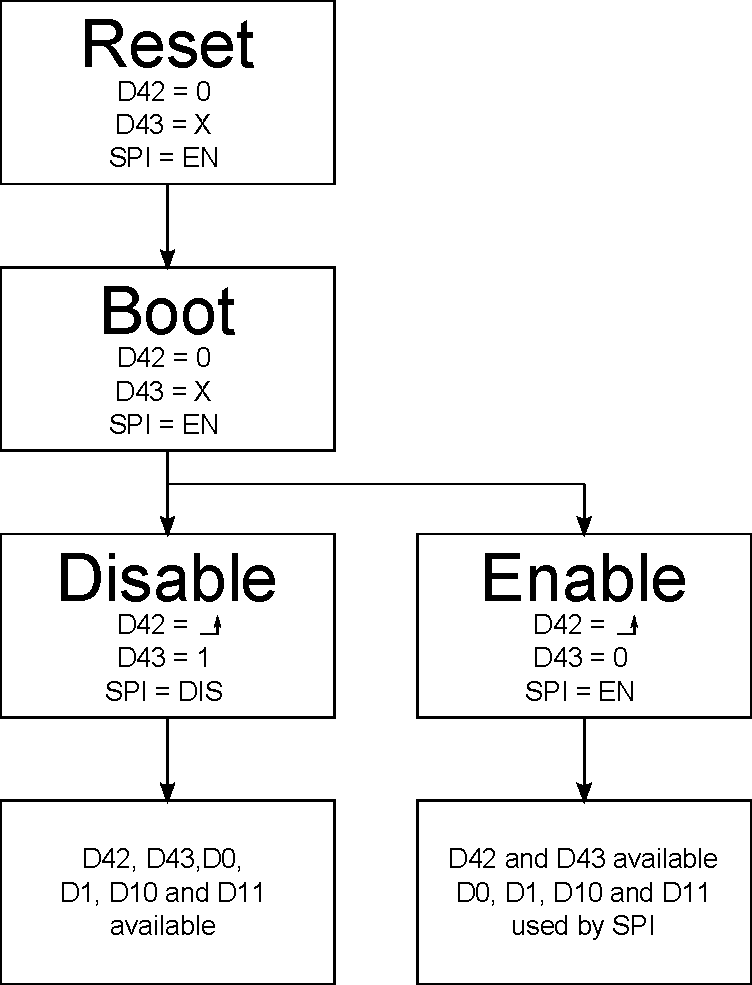
\includegraphics[width=0.500\linewidth]{spiselectflow.pdf}
\end{sidecaption}\end{figure} \DocumentFooterFix


Once this sequence is completed the selection has been latched, therefore X0D42 and X0D43 return to performing their normal functions in the \verb`Triangle` slot.


If\attentionmargin  the SPI is not disabled, then Slice Cards in the \verb`Star`, \verb`Triangle` or \verb`A` slots may not function as expected. If there are no Slice Cards in the \verb`Star`, \verb`Triangle` or \verb`A` slot, then it does not matter whether the SPI has been disabled or not. Therefore, applications which require runtime access to the SPI flash should either leave the \verb`Star`, \verb`Triangle` and \verb`A` slots unpopulated or check to ensure that the Card which is in there will be unaffected by the operation of the Flash.


The xTAG debug system can use the boot mode select signal to force all devices in the chain (master and slave Core Boards) to boot from JTAG (don't boot) for debug purposes.


If not in this mode, the devices will boot from SPI or xCONNECT link as appropriate.



% NON-FULLWIDTH SECTION
\section{xCONNECT Links}
\label{a16_core_board:xconnect-links}

The Chain Connector contains two 5-bit xCONNECT links, XLA and XLB, which can be used for chaining sliceKIT Core Boards together. The links from Tile 0 are connected to the \verb`Chain` Connector and the \verb`Star` Slot.  The links from Tile 1 are connected to the \verb`Square` Slot.


The only complication in this system is use of the xSCOPE 2-bit xCONNECT Link. This link overlaps a 4 bit port on the \verb`Star` Slot connector so it would not be possible to use this for user I/O at the same time as xSCOPE.


To work around this, a switch is present on the XSYS adapter board to either enable or disable the xSCOPE xCONNECT Link.


When disabled, these pins are disconnected from the \verb`Chain` Connector and are free for use on the \verb`Star` Slot. When enabled they will work as an xCONNECT link and hence will appear on the relevant pins of the \verb`Star` Slot.


It\attentionmargin  is recommended that if a sliceCARD is used in the \verb`Star` Slot the xSCOPE switch is off on the XSYS Adaptor Card to ensure correct operation of the sliceCARD in the \verb`Star` slot.



% NON-FULLWIDTH SECTION
\section{Reset}
\label{a16_core_board:reset}

The whole system is held in reset until all power supplies are stable, and reset is connected to all Slice Cards so any circuitry on them can be reset.


It also indicates to the sliceCARDs that their power input is stable. The reset from the xTAG resets the whole system, if required for debugging.



% NON-FULLWIDTH SECTION
\section{Clocking}
\label{a16_core_board:clocking}

There are two sources for the system clock: an on-board 25MHz oscillator or the CLK signal from the \verb`Chain` Connector. The system clock source is selected automatically according to the presence signals on the \verb`Chain` connector.


This means the system clock from a Master Core Board is fed automatically to all of the slave Core Boards so the whole system will operate synchronously.


The system clock is also fed to each of the sliceCARD Slots.



% NON-FULLWIDTH SECTION
\section{Testpoints}
\label{a16_core_board:testpoints}\label{a16_core_board:sec-io-crossref}

Each xCORE I/O signal is also available on a 0.1'' header, next to the Slot that it is connected to.


These connections can be used to connect an oscilloscope or logic analyser, or for interconnection of signals for advanced development work.


The signals are identified on the silkscreen layer of the sliceKIT Core Board, the table below lists their relationship to the internal ports.

\small\begin{longtable}{llllllll}
\Toprule
\endfirsthead

\Toprule
\textbf{A16 Pin} & \textbf{Slot} & \textbf{PCIE} & \multicolumn{5}{>{\setlength{\hsize}{5\hsize}\addtolength{\hsize}{5\tabcolsep}}l}{\textbf{Function}}\\
\midrule


\endhead

 \multicolumn{8}{r}{{(continued)}} \\ 
\endfoot


\endlastfoot

\textbf{A16 Pin} & \textbf{Slot} & \textbf{PCIE} & \multicolumn{5}{>{\setlength{\hsize}{5\hsize}\addtolength{\hsize}{5\tabcolsep}}l}{\textbf{Function}}\\
\midrule
X0D0 & TRIANGLE & B2 & P1A0 &  &  &  & \\
X0D1 & STAR & A8 & P1B0 &  &  &  & \\
 & MIXED SIG & B15 &  &  &  &  & \\
 & CHAIN & B10 &  &  &  &  & \\
X0D2 & STAR & B6 &  & P4A0 & P8A0 & P16A0 & P32A20\\
 & CHAIN & A7 &  &  &  &  & \\
X0D3 & STAR & B7 &  & P4A1 & P8A1 & P16A1 & P32A21\\
 & CHAIN & A6 &  &  &  &  & \\
X0D4 & STAR & B9 &  & P4B0 & P8A2 & P16A2 & P32A22\\
 & CHAIN & A11 &  &  &  &  & \\
X0D5 & STAR & B11 &  & P4B1 & P8A3 & P16A3 & P32A23\\
 & CHAIN & A9 &  &  &  &  & \\
X0D6 & STAR & A9 &  & P4B2 & P8A4 & P16A4 & P32A24\\
 & CHAIN & B11 &  &  &  &  & \\
X0D7 & STAR & A11 &  & P4B3 & P8A5 & P16A5 & P32A25\\
 & CHAIN & B9 &  &  &  &  & \\
X0D8 & STAR & A6 &  & P4A2 & P8A6 & P16A6 & P32A26\\
 & CHAIN & B7 &  &  &  &  & \\
X0D9 & STAR & A7 &  & P4A3 & P8A7 & P16A7 & P32A27\\
 & CHAIN & B6 &  &  &  &  & \\
X0D10 & STAR & B10 & P1C0 &  &  &  & \\
 & MIXED SIG & B2 &  &  &  &  & \\
 & CHAIN & A8 &  &  &  &  & \\
X0D11 & TRIANGLE & B4 & P1D0 &  &  &  & \\
X0D12 & TRIANGLE & A3 & P1E0 &  &  &  & \\
X0D13 & STAR & A15 & P1F0 &  &  &  & \\
 & MIXED SIG & A3 &  &  &  &  & \\
 & CHAIN & B15 &  &  &  &  & \\
X0D14 & STAR & B12 &  & P4C0 & P8B0 & P16A8 & P32A28\\
 & CHAIN & A13 &  &  &  &  & \\
X0D15 & STAR & B13 &  & P4C1 & P8B1 & P16A9 & P32A29\\
 & CHAIN & A12 &  &  &  &  & \\
X0D16 & STAR & B17 &  & P4D0 & P8B2 & P16A10 & \\
 & CHAIN & A18 &  &  &  &  & \\
X0D17 & STAR & B18 &  & P4D1 & P8B3 & P16A11 & \\
 & CHAIN & A17 &  &  &  &  & \\
X0D18 & STAR & A17 &  & P4D2 & P8B4 & P16A12 & \\
 & CHAIN & B18 &  &  &  &  & \\
X0D19 & STAR & A18 &  & P4D3 & P8B5 & P16A13 & \\
 & CHAIN & B17 &  &  &  &  & \\
X0D20 & STAR & A12 &  & P4C2 & P8B6 & P16A14 & P32A30\\
 & CHAIN & B13 &  &  &  &  & \\
X0D21 & STAR & A13 &  & P4C3 & P8B7 & P16A15 & P32A31\\
 & CHAIN & B12 &  &  &  &  & \\
X0D22 & STAR & B15 & P1G0 &  &  &  & \\
 & MIXED SIG & B4 &  &  &  &  & \\
 & CHAIN & A15 &  &  &  &  & \\
X0D23 & TRIANGLE & A4 & P1H0 &  &  &  & \\
X0D24 & TRIANGLE & B15 & P1I0 &  &  &  & \\
X0D25 & TRIANGLE & A8 & P1J0 &  &  &  & \\
X0D26 & TRIANGLE & B6 &  & P4E0 & P8C0 & P16B0 & \\
X0D27 & TRIANGLE & B7 &  & P4E1 & P8C1 & P16B1 & \\
X0D28 & TRIANGLE & B9 &  & P4F0 & P8C2 & P16B2 & \\
X0D29 & TRIANGLE & B11 &  & P4F1 & P8C3 & P16B3 & \\
X0D30 & TRIANGLE & A9 &  & P4F2 & P8C4 & P16B4 & \\
X0D31 & TRIANGLE & A11 &  & P4F3 & P8C5 & P16B5 & \\
X0D32 & TRIANGLE & A6 &  & P4E2 & P8C6 & P16B6 & \\
X0D33 & TRIANGLE & A7 &  & P4E3 & P8C7 & P16B7 & \\
X0D34 & TRIANGLE & B10 & P1K0 &  &  &  & \\
X0D35 & TRIANGLE & A15 & P1L0 &  &  &  & \\
X0D36 & TRIANGLE & B12 & P1M0 &  & P8D0 & P16B8 & \\
X0D37 & TRIANGLE & B13 & P1N0 &  & P8D1 & P16B9 & \\
X0D38 & TRIANGLE & B17 & P1O0 &  & P8D2 & P16B10 & \\
X0D39 & TRIANGLE & B18 & P1P0 &  & P8D3 & P16B11 & \\
X0D40 & TRIANGLE & A17 &  &  & P8D4 & P16B12 & \\
X0D41 & TRIANGLE & A18 &  &  & P8D5 & P16B13 & \\
X0D42 & TRIANGLE & A12 &  &  & P8D6 & P16B14 & \\
X0D43 & TRIANGLE & A13 &  &  & P8D7 & P16B15 & \\
 & MIXED SIG & A4 &  &  &  &  & \\
X1D0 & CIRCLE & B2 & P1A0 &  &  &  & \\
X1D1 & SQUARE & A8 & P1B0 &  &  &  & \\
X1D2 & SQUARE & B6 &  & P4A0 & P8A0 & P16A0 & P32A20\\
X1D3 & SQUARE & B7 &  & P4A1 & P8A1 & P16A1 & P32A21\\
X1D4 & SQUARE & B9 &  & P4B0 & P8A2 & P16A2 & P32A22\\
X1D5 & SQUARE & B11 &  & P4B1 & P8A3 & P16A3 & P32A23\\
X1D6 & SQUARE & A9 &  & P4B2 & P8A4 & P16A4 & P32A24\\
X1D7 & SQUARE & A11 &  & P4B3 & P8A5 & P16A5 & P32A25\\
X1D8 & SQUARE & A6 &  & P4A2 & P8A6 & P16A6 & P32A26\\
X1D9 & SQUARE & A7 &  & P4A3 & P8A7 & P16A7 & P32A27\\
X1D10 & SQUARE & B10 & P1C0 &  &  &  & \\
X1D11 & CIRCLE & B4 & P1D0 &  &  &  & \\
X1D12 & CIRCLE & A3 & P1E0 &  &  &  & \\
X1D13 & SQUARE & A15 & P1F0 &  &  &  & \\
X1D14 & SQUARE & B12 &  & P4C0 & P8B0 & P16A8 & P32A28\\
X1D15 & SQUARE & B13 &  & P4C1 & P8B1 & P16A9 & P32A29\\
X1D16 & SQUARE & B17 &  & P4D0 & P8B2 & P16A10 & \\
X1D17 & SQUARE & B18 &  & P4D1 & P8B3 & P16A11 & \\
X1D18 & SQUARE & A17 &  & P4D2 & P8B4 & P16A12 & \\
X1D19 & SQUARE & A18 &  & P4D3 & P8B5 & P16A13 & \\
X1D20 & SQUARE & A12 &  & P4C2 & P8B6 & P16A14 & P32A30\\
X1D21 & SQUARE & A13 &  & P4C3 & P8B7 & P16A15 & P32A31\\
X1D22 & SQUARE & B15 & P1G0 &  &  &  & \\
X1D23 & CIRCLE & A4 & P1H0 &  &  &  & \\
X1D24 & CIRCLE & B15 & P1I0 &  &  &  & \\
X1D25 & CIRCLE & A8 & P1J0 &  &  &  & \\
X1D26 & CIRCLE & B6 &  & P4E0 & P8C0 & P16B0 & \\
X1D27 & CIRCLE & B7 &  & P4E1 & P8C1 & P16B1 & \\
X1D28 & CIRCLE & B9 &  & P4F0 & P8C2 & P16B2 & \\
X1D29 & CIRCLE & B11 &  & P4F1 & P8C3 & P16B3 & \\
X1D30 & CIRCLE & A9 &  & P4F2 & P8C4 & P16B4 & \\
X1D31 & CIRCLE & A11 &  & P4F3 & P8C5 & P16B5 & \\
X1D32 & CIRCLE & A6 &  & P4E2 & P8C6 & P16B6 & \\
X1D33 & CIRCLE & A7 &  & P4E3 & P8C7 & P16B7 & \\
X1D34 & CIRCLE & B10 & P1K0 &  &  &  & \\
X1D35 & CIRCLE & A15 & P1L0 &  &  &  & \\
X1D36 & CIRCLE & B12 & P1M0 &  & P8D0 & P16B8 & \\
X1D37 & CIRCLE & B13 & P1N0 &  & P8D1 & P16B9 & \\
X1D38 & CIRCLE & B17 & P1O0 &  & P8D2 & P16B10 & \\
X1D39 & CIRCLE & B18 & P1P0 &  & P8D3 & P16B11 & \\
X1D40 & CIRCLE & A17 &  &  & P8D4 & P16B12 & \\
X1D41 & CIRCLE & A18 &  &  & P8D5 & P16B13 & \\
X1D42 & CIRCLE & A12 &  &  & P8D6 & P16B14 & \\
X1D43 & CIRCLE & A13 &  &  & P8D7 & P16B15 & \\
\bottomrule
\end{longtable}

\normalsize



% NON-FULLWIDTH SECTION
\section{Slot pinouts}
\label{a16_core_board:slot-pinouts}

The signal assignments for the connectors on the Core Board and sliceCARDs can be seen in the table below.



% NON-FULLWIDTH SECTION
\subsection{STAR}
\label{a16_core_board:star}
\begin{tabular}{lllllll}
\Toprule
\textbf{PCIE B (TOP)} & \textbf{SIGNAL} & \multicolumn{5}{>{\setlength{\hsize}{5\hsize}\addtolength{\hsize}{5\tabcolsep}}l}{\textbf{FUNCTION}}\\
\midrule
B1 & NC & \multicolumn{5}{>{\setlength{\hsize}{5\hsize}\addtolength{\hsize}{5\tabcolsep}}l}{NOT CONNECTED}\\
B2 & NC & \multicolumn{5}{>{\setlength{\hsize}{5\hsize}\addtolength{\hsize}{5\tabcolsep}}l}{NOT CONNECTED}\\
B3 & \emph{GND} & \multicolumn{5}{>{\setlength{\hsize}{5\hsize}\addtolength{\hsize}{5\tabcolsep}}l}{POWER SUPPLY GROUND}\\
B4 & NC & \multicolumn{5}{>{\setlength{\hsize}{5\hsize}\addtolength{\hsize}{5\tabcolsep}}l}{NOT CONNECTED}\\
B5 & \emph{3V3} & \multicolumn{5}{>{\setlength{\hsize}{5\hsize}\addtolength{\hsize}{5\tabcolsep}}l}{POWER SUPPLY 3.3V}\\
B6 & X0D2 &  & P4A0 & P8A0 & P16A0 & P32A20\\
B7 & X0D3 &  & P4A1 & P8A1 & P16A1 & P32A21\\
B8 & \emph{GND} & \multicolumn{5}{>{\setlength{\hsize}{5\hsize}\addtolength{\hsize}{5\tabcolsep}}l}{POWER SUPPLY GROUND}\\
B9 & X0D4 &  & P4B0 & P8A2 & P16A2 & P32A22\\
B10 & X0D10 & P1C0 &  &  &  & \\
B11 & X0D5 &  & P4B1 & P8A3 & P16A3 & P32A23\\
\textbf{KEY} & \textbf{KEY} & \multicolumn{5}{>{\setlength{\hsize}{5\hsize}\addtolength{\hsize}{5\tabcolsep}}l}{\textbf{MECHANICAL KEY}}\\
B12 & X0D14 &  & P4C0 & P8B0 & P16A8 & P32A28\\
B13 & X0D15 &  & P4C1 & P8B1 & P16A9 & P32A29\\
B14 & \emph{CLK} & \multicolumn{5}{>{\setlength{\hsize}{5\hsize}\addtolength{\hsize}{5\tabcolsep}}l}{MAIN SYSTEM CLOCK}\\
B15 & X0D22 & P1G0 &  &  &  & \\
B16 & \emph{GND} & \multicolumn{5}{>{\setlength{\hsize}{5\hsize}\addtolength{\hsize}{5\tabcolsep}}l}{POWER SUPPLY GROUND}\\
B17 & X0D16 &  & P4D0 & P8B2 & P16A10 & \\
B18 & X0D17 &  & P4D1 & P8B3 & P16A11 & \\
\bottomrule
\end{tabular}


\begin{tabular}{lllllll}
\Toprule
\textbf{PCIE A (BOT)} & \textbf{SIGNAL} & \multicolumn{5}{>{\setlength{\hsize}{5\hsize}\addtolength{\hsize}{5\tabcolsep}}l}{\textbf{FUNCTION}}\\
\midrule
A1 & NC & \multicolumn{5}{>{\setlength{\hsize}{5\hsize}\addtolength{\hsize}{5\tabcolsep}}l}{NOT CONNECTED}\\
A2 & \emph{5V} & \multicolumn{5}{>{\setlength{\hsize}{5\hsize}\addtolength{\hsize}{5\tabcolsep}}l}{POWER SUPPLY 5V}\\
A3 & NC & \multicolumn{5}{>{\setlength{\hsize}{5\hsize}\addtolength{\hsize}{5\tabcolsep}}l}{NOT CONNECTED}\\
A4 & NC & \multicolumn{5}{>{\setlength{\hsize}{5\hsize}\addtolength{\hsize}{5\tabcolsep}}l}{NOT CONNECTED}\\
A5 & \emph{GND} & \multicolumn{5}{>{\setlength{\hsize}{5\hsize}\addtolength{\hsize}{5\tabcolsep}}l}{POWER SUPPLY GROUND}\\
A6 & X0D8 &  & P4A2 & P8A6 & P16A6 & P32A26\\
A7 & X0D9 &  & P4A3 & P8A7 & P16A7 & P32A27\\
A8 & X0D1 & P1B0 &  &  &  & \\
A9 & X0D6 &  & P4B2 & P8A4 & P16A4 & P32A24\\
A10 & \emph{GND} & \multicolumn{5}{>{\setlength{\hsize}{5\hsize}\addtolength{\hsize}{5\tabcolsep}}l}{POWER SUPPLY GROUND}\\
A11 & X0D7 &  & P4B3 & P8A5 & P16A5 & P32A25\\
\textbf{KEY} & \textbf{KEY} & \multicolumn{5}{>{\setlength{\hsize}{5\hsize}\addtolength{\hsize}{5\tabcolsep}}l}{\textbf{MECHANICAL KEY}}\\
A12 & X0D20 &  & P4C2 & P8B6 & P16A14 & P32A30\\
A13 & X0D21 &  & P4C3 & P8B7 & P16A15 & P32A31\\
A14 & \emph{GND} & \multicolumn{5}{>{\setlength{\hsize}{5\hsize}\addtolength{\hsize}{5\tabcolsep}}l}{POWER SUPPLY GROUND}\\
A15 & X0D13 & P1F0 &  &  &  & \\
A16 & \emph{RST\_N} & \multicolumn{5}{>{\setlength{\hsize}{5\hsize}\addtolength{\hsize}{5\tabcolsep}}l}{SYSTEM RESET (ACTIVE LOW)}\\
A17 & X0D18 &  & P4D2 & P8B4 & P16A12 & \\
A18 & X0D19 &  & P4D3 & P8B5 & P16A13 & \\
\bottomrule
\end{tabular}




% NON-FULLWIDTH SECTION
\subsection{SQUARE}
\label{a16_core_board:square}
\begin{tabular}{lllllll}
\Toprule
\textbf{PCIE B (TOP)} & \textbf{SIGNAL} & \multicolumn{5}{>{\setlength{\hsize}{5\hsize}\addtolength{\hsize}{5\tabcolsep}}l}{\textbf{FUNCTION}}\\
\midrule
B1 & \emph{DEBUG} & \multicolumn{5}{>{\setlength{\hsize}{5\hsize}\addtolength{\hsize}{5\tabcolsep}}l}{XSYS DEBUG SIGNAL}\\
B2 & \emph{TCK} & \multicolumn{5}{>{\setlength{\hsize}{5\hsize}\addtolength{\hsize}{5\tabcolsep}}l}{XSYS TCK SIGNAL}\\
B3 & \emph{GND} & \multicolumn{5}{>{\setlength{\hsize}{5\hsize}\addtolength{\hsize}{5\tabcolsep}}l}{POWER SUPPLY GROUND}\\
B4 & \emph{TDI} & \multicolumn{5}{>{\setlength{\hsize}{5\hsize}\addtolength{\hsize}{5\tabcolsep}}l}{XSYS TDI SIGNAL}\\
B5 & \emph{3V3} & \multicolumn{5}{>{\setlength{\hsize}{5\hsize}\addtolength{\hsize}{5\tabcolsep}}l}{POWER SUPPLY 3.3V}\\
B6 & X1D2 &  & P4A0 & P8A0 & P16A0 & P32A20\\
B7 & X1D3 &  & P4A1 & P8A1 & P16A1 & P32A21\\
B8 & \emph{GND} & \multicolumn{5}{>{\setlength{\hsize}{5\hsize}\addtolength{\hsize}{5\tabcolsep}}l}{POWER SUPPLY GROUND}\\
B9 & X1D4 &  & P4B0 & P8A2 & P16A2 & P32A22\\
B10 & X1D10 & P1C0 &  &  &  & \\
B11 & X1D5 &  & P4B1 & P8A3 & P16A3 & P32A23\\
\textbf{KEY} & \textbf{KEY} & \multicolumn{5}{>{\setlength{\hsize}{5\hsize}\addtolength{\hsize}{5\tabcolsep}}l}{\textbf{MECHANICAL KEY}}\\
B12 & X1D14 &  & P4C0 & P8B0 & P16A8 & P32A28\\
B13 & X1D15 &  & P4C1 & P8B1 & P16A9 & P32A29\\
B14 & \emph{CLK} & \multicolumn{5}{>{\setlength{\hsize}{5\hsize}\addtolength{\hsize}{5\tabcolsep}}l}{MAIN SYSTEM CLOCK}\\
B15 & X1D22 & P1G0 &  &  &  & \\
B16 & \emph{GND} & \multicolumn{5}{>{\setlength{\hsize}{5\hsize}\addtolength{\hsize}{5\tabcolsep}}l}{POWER SUPPLY GROUND}\\
B17 & X1D16 &  & P4D0 & P8B2 & P16A10 & \\
B18 & X1D17 &  & P4D1 & P8B3 & P16A11 & \\
\bottomrule
\end{tabular}


\begin{tabular}{lllllll}
\Toprule
\textbf{PCIE A (BOT)} & \textbf{SIGNAL} & \multicolumn{5}{>{\setlength{\hsize}{5\hsize}\addtolength{\hsize}{5\tabcolsep}}l}{\textbf{FUNCTION}}\\
\midrule
A1 & \emph{MSEL} & \multicolumn{5}{>{\setlength{\hsize}{5\hsize}\addtolength{\hsize}{5\tabcolsep}}l}{XSYS MSEL SIGNAL}\\
A2 & \emph{5V} & \multicolumn{5}{>{\setlength{\hsize}{5\hsize}\addtolength{\hsize}{5\tabcolsep}}l}{POWER SUPPLY 5V}\\
A3 & \emph{TMS} & \multicolumn{5}{>{\setlength{\hsize}{5\hsize}\addtolength{\hsize}{5\tabcolsep}}l}{XSYS TMS SIGNAL}\\
A4 & \emph{TDO} & \multicolumn{5}{>{\setlength{\hsize}{5\hsize}\addtolength{\hsize}{5\tabcolsep}}l}{XSYS TDO SIGNAL}\\
A5 & \emph{PRSNT} & \multicolumn{5}{>{\setlength{\hsize}{5\hsize}\addtolength{\hsize}{5\tabcolsep}}l}{SYSTEM PRESENT SIGNAL (ACTIVE LOW)}\\
A6 & X1D8 &  & P4A2 & P8A6 & P16A6 & P32A26\\
A7 & X1D9 &  & P4A3 & P8A7 & P16A7 & P32A27\\
A8 & X1D1 & P1B0 &  &  &  & \\
A9 & X1D6 &  & P4B2 & P8A4 & P16A4 & P32A24\\
A10 & \emph{GND} & \multicolumn{5}{>{\setlength{\hsize}{5\hsize}\addtolength{\hsize}{5\tabcolsep}}l}{POWER SUPPLY GROUND}\\
A11 & X1D7 &  & P4B3 & P8A5 & P16A5 & P32A25\\
\textbf{KEY} & \textbf{KEY} & \multicolumn{5}{>{\setlength{\hsize}{5\hsize}\addtolength{\hsize}{5\tabcolsep}}l}{\textbf{MECHANICAL KEY}}\\
A12 & X1D20 &  & P4C2 & P8B6 & P16A14 & P32A30\\
A13 & X1D21 &  & P4C3 & P8B7 & P16A15 & P32A31\\
A14 & \emph{GND} & \multicolumn{5}{>{\setlength{\hsize}{5\hsize}\addtolength{\hsize}{5\tabcolsep}}l}{POWER SUPPLY GROUND}\\
A15 & X1D13 & P1F0 &  &  &  & \\
A16 & \emph{RST\_N} & \multicolumn{5}{>{\setlength{\hsize}{5\hsize}\addtolength{\hsize}{5\tabcolsep}}l}{SYSTEM RESET (ACTIVE LOW)}\\
A17 & X1D18 &  & P4D2 & P8B4 & P16A12 & \\
A18 & X1D19 &  & P4D3 & P8B5 & P16A13 & \\
\bottomrule
\end{tabular}




% NON-FULLWIDTH SECTION
\subsection{TRIANGLE}
\label{a16_core_board:triangle}
\begin{tabular}{lllllll}
\Toprule
\textbf{PCIE B (TOP)} & \textbf{SIGNAL} & \multicolumn{5}{>{\setlength{\hsize}{5\hsize}\addtolength{\hsize}{5\tabcolsep}}l}{\textbf{FUNCTION}}\\
\midrule
B1 & NC & \multicolumn{5}{>{\setlength{\hsize}{5\hsize}\addtolength{\hsize}{5\tabcolsep}}l}{NOT CONNECTED}\\
B2 & X0D0 & P1A0 &  &  &  & \\
B3 & \emph{GND} & \multicolumn{5}{>{\setlength{\hsize}{5\hsize}\addtolength{\hsize}{5\tabcolsep}}l}{POWER SUPPLY GROUND}\\
B4 & X0D11 & P1D0 &  &  &  & \\
B5 & \emph{3V3} & \multicolumn{5}{>{\setlength{\hsize}{5\hsize}\addtolength{\hsize}{5\tabcolsep}}l}{POWER SUPPLY 3.3V}\\
B6 & X0D26 &  & P4E0 & P8C0 & P16B0 & \\
B7 & X0D27 &  & P4E1 & P8C1 & P16B1 & \\
B8 & \emph{GND} & \multicolumn{5}{>{\setlength{\hsize}{5\hsize}\addtolength{\hsize}{5\tabcolsep}}l}{POWER SUPPLY GROUND}\\
B9 & X0D28 &  & P4F0 & P8C2 & P16B2 & \\
B10 & X0D34 & P1K0 &  &  &  & \\
B11 & X0D29 &  & P4F1 & P8C3 & P16B3 & \\
\textbf{KEY} & \textbf{KEY} & \multicolumn{5}{>{\setlength{\hsize}{5\hsize}\addtolength{\hsize}{5\tabcolsep}}l}{\textbf{MECHANICAL KEY}}\\
B12 & X0D36 & P1M0 &  & P8D0 & P16B8 & \\
B13 & X0D37 & P1N0 &  & P8D1 & P16B9 & \\
B14 & \emph{CLK} & \multicolumn{5}{>{\setlength{\hsize}{5\hsize}\addtolength{\hsize}{5\tabcolsep}}l}{MAIN SYSTEM CLOCK}\\
B15 & X0D24 & P1I0 &  &  &  & \\
B16 & \emph{GND} & \multicolumn{5}{>{\setlength{\hsize}{5\hsize}\addtolength{\hsize}{5\tabcolsep}}l}{POWER SUPPLY GROUND}\\
B17 & X0D38 & P1O0 &  & P8D2 & P16B10 & \\
B18 & X0D39 & P1P0 &  & P8D3 & P16B11 & \\
\bottomrule
\end{tabular}


\begin{tabular}{lllllll}
\Toprule
\textbf{PCIE A (BOT)} & \textbf{SIGNAL} & \multicolumn{5}{>{\setlength{\hsize}{5\hsize}\addtolength{\hsize}{5\tabcolsep}}l}{\textbf{FUNCTION}}\\
\midrule
A1 & NC & \multicolumn{5}{>{\setlength{\hsize}{5\hsize}\addtolength{\hsize}{5\tabcolsep}}l}{NOT CONNECTED}\\
A2 & \emph{5V} & \multicolumn{5}{>{\setlength{\hsize}{5\hsize}\addtolength{\hsize}{5\tabcolsep}}l}{POWER SUPPLY 5V}\\
A3 & X0D12 & P1E0 &  &  &  & \\
A4 & X0D23 & P1H0 &  &  &  & \\
A5 & \emph{GND} & \multicolumn{5}{>{\setlength{\hsize}{5\hsize}\addtolength{\hsize}{5\tabcolsep}}l}{POWER SUPPLY GROUND}\\
A6 & X0D32 &  & P4E2 & P8C6 & P16B6 & \\
A7 & X0D33 &  & P4E3 & P8C7 & P16B7 & \\
A8 & X0D25 & P1J0 &  &  &  & \\
A9 & X0D30 &  & P4F2 & P8C4 & P16B4 & \\
A10 & \emph{GND} & \multicolumn{5}{>{\setlength{\hsize}{5\hsize}\addtolength{\hsize}{5\tabcolsep}}l}{POWER SUPPLY GROUND}\\
A11 & X0D31 &  & P4F3 & P8C5 & P16B5 & \\
\textbf{KEY} & \textbf{KEY} & \multicolumn{5}{>{\setlength{\hsize}{5\hsize}\addtolength{\hsize}{5\tabcolsep}}l}{\textbf{MECHANICAL KEY}}\\
A12 & X0D42 &  &  & P8D6 & P16B14 & \\
A13 & X0D43 &  &  & P8D7 & P16B15 & \\
A14 & \emph{GND} & \multicolumn{5}{>{\setlength{\hsize}{5\hsize}\addtolength{\hsize}{5\tabcolsep}}l}{POWER SUPPLY GROUND}\\
A15 & X0D35 & P1L0 &  &  &  & \\
A16 & \emph{RST\_N} & \multicolumn{5}{>{\setlength{\hsize}{5\hsize}\addtolength{\hsize}{5\tabcolsep}}l}{SYSTEM RESET (ACTIVE LOW)}\\
A17 & X0D40 &  &  & P8D4 & P16B12 & \\
A18 & X0D41 &  &  & P8D5 & P16B13 & \\
\bottomrule
\end{tabular}




% NON-FULLWIDTH SECTION
\subsection{CIRCLE}
\label{a16_core_board:circle}
\begin{tabular}{lllllll}
\Toprule
\textbf{PCIE B (TOP)} & \textbf{SIGNAL} & \multicolumn{5}{>{\setlength{\hsize}{5\hsize}\addtolength{\hsize}{5\tabcolsep}}l}{\textbf{FUNCTION}}\\
\midrule
B1 & NC & \multicolumn{5}{>{\setlength{\hsize}{5\hsize}\addtolength{\hsize}{5\tabcolsep}}l}{NOT CONNECTED}\\
B2 & X1D0 & P1A0 &  &  &  & \\
B3 & \emph{GND} & \multicolumn{5}{>{\setlength{\hsize}{5\hsize}\addtolength{\hsize}{5\tabcolsep}}l}{POWER SUPPLY GROUND}\\
B4 & X1D11 & P1D0 &  &  &  & \\
B5 & \emph{3V3} & \multicolumn{5}{>{\setlength{\hsize}{5\hsize}\addtolength{\hsize}{5\tabcolsep}}l}{POWER SUPPLY 3.3V}\\
B6 & X1D26 &  & P4E0 & P8C0 & P16B0 & \\
B7 & X1D27 &  & P4E1 & P8C1 & P16B1 & \\
B8 & \emph{GND} & \multicolumn{5}{>{\setlength{\hsize}{5\hsize}\addtolength{\hsize}{5\tabcolsep}}l}{POWER SUPPLY GROUND}\\
B9 & X1D28 &  & P4F0 & P8C2 & P16B2 & \\
B10 & X1D34 & P1K0 &  &  &  & \\
B11 & X1D29 &  & P4F1 & P8C3 & P16B3 & \\
\textbf{KEY} & \textbf{KEY} & \multicolumn{5}{>{\setlength{\hsize}{5\hsize}\addtolength{\hsize}{5\tabcolsep}}l}{\textbf{MECHANICAL KEY}}\\
B12 & X1D36 & P1M0 &  & P8D0 & P16B8 & \\
B13 & X1D37 & P1N0 &  & P8D1 & P16B9 & \\
B14 & \emph{CLK} & \multicolumn{5}{>{\setlength{\hsize}{5\hsize}\addtolength{\hsize}{5\tabcolsep}}l}{MAIN SYSTEM CLOCK}\\
B15 & X1D24 & P1I0 &  &  &  & \\
B16 & \emph{GND} & \multicolumn{5}{>{\setlength{\hsize}{5\hsize}\addtolength{\hsize}{5\tabcolsep}}l}{POWER SUPPLY GROUND}\\
B17 & X1D38 & P1O0 &  & P8D2 & P16B10 & \\
B18 & X1D39 & P1P0 &  & P8D3 & P16B11 & \\
\bottomrule
\end{tabular}


\begin{tabular}{lllllll}
\Toprule
\textbf{PCIE A (BOT)} & \textbf{SIGNAL} & \multicolumn{5}{>{\setlength{\hsize}{5\hsize}\addtolength{\hsize}{5\tabcolsep}}l}{\textbf{FUNCTION}}\\
\midrule
A1 & NC & \multicolumn{5}{>{\setlength{\hsize}{5\hsize}\addtolength{\hsize}{5\tabcolsep}}l}{NOT CONNECTED}\\
A2 & \emph{5V} & \multicolumn{5}{>{\setlength{\hsize}{5\hsize}\addtolength{\hsize}{5\tabcolsep}}l}{POWER SUPPLY 5V}\\
A3 & X1D12 & P1E0 &  &  &  & \\
A4 & X1D23 & P1H0 &  &  &  & \\
A5 & \emph{GND} & \multicolumn{5}{>{\setlength{\hsize}{5\hsize}\addtolength{\hsize}{5\tabcolsep}}l}{POWER SUPPLY GROUND}\\
A6 & X1D32 &  & P4E2 & P8C6 & P16B6 & \\
A7 & X1D33 &  & P4E3 & P8C7 & P16B7 & \\
A8 & X1D25 & P1J0 &  &  &  & \\
A9 & X1D30 &  & P4F2 & P8C4 & P16B4 & \\
A10 & \emph{GND} & \multicolumn{5}{>{\setlength{\hsize}{5\hsize}\addtolength{\hsize}{5\tabcolsep}}l}{POWER SUPPLY GROUND}\\
A11 & X1D31 &  & P4F3 & P8C5 & P16B5 & \\
\textbf{KEY} & \textbf{KEY} & \multicolumn{5}{>{\setlength{\hsize}{5\hsize}\addtolength{\hsize}{5\tabcolsep}}l}{\textbf{MECHANICAL KEY}}\\
A12 & X1D42 &  &  & P8D6 & P16B14 & \\
A13 & X1D43 &  &  & P8D7 & P16B15 & \\
A14 & \emph{GND} & \multicolumn{5}{>{\setlength{\hsize}{5\hsize}\addtolength{\hsize}{5\tabcolsep}}l}{POWER SUPPLY GROUND}\\
A15 & X1D35 & P1L0 &  &  &  & \\
A16 & \emph{RST\_N} & \multicolumn{5}{>{\setlength{\hsize}{5\hsize}\addtolength{\hsize}{5\tabcolsep}}l}{SYSTEM RESET (ACTIVE LOW)}\\
A17 & X1D40 &  &  & P8D4 & P16B12 & \\
A18 & X1D41 &  &  & P8D5 & P16B13 & \\
\bottomrule
\end{tabular}




% NON-FULLWIDTH SECTION
\subsection{CHAIN}
\label{a16_core_board:chain}
\begin{tabular}{lllllll}
\Toprule
\textbf{PCIE B (TOP)} & \textbf{SIGNAL} & \multicolumn{5}{>{\setlength{\hsize}{5\hsize}\addtolength{\hsize}{5\tabcolsep}}l}{\textbf{FUNCTION}}\\
\midrule
B1 & DEBUG & \multicolumn{5}{>{\setlength{\hsize}{5\hsize}\addtolength{\hsize}{5\tabcolsep}}l}{XSYS DEBUG SINGAL}\\
B2 & TCK & \multicolumn{5}{>{\setlength{\hsize}{5\hsize}\addtolength{\hsize}{5\tabcolsep}}l}{XSYS TCK SIGNAL}\\
B3 & \emph{GND} & \multicolumn{5}{>{\setlength{\hsize}{5\hsize}\addtolength{\hsize}{5\tabcolsep}}l}{POWER SUPPLY GROUND}\\
B4 & TDO & \multicolumn{5}{>{\setlength{\hsize}{5\hsize}\addtolength{\hsize}{5\tabcolsep}}l}{XSYS TDO SIGNAL}\\
B5 & PRSNT & \multicolumn{5}{>{\setlength{\hsize}{5\hsize}\addtolength{\hsize}{5\tabcolsep}}l}{CHAIN PRESENT SIGNAL}\\
B6 & X0D9 & XLA4o &  & XLA5b &  & \\
B7 & X0D8 & XLA2i &  & XLA5b &  & \\
B8 & \emph{GND} & \multicolumn{5}{>{\setlength{\hsize}{5\hsize}\addtolength{\hsize}{5\tabcolsep}}l}{POWER SUPPLY GROUND}\\
B9 & X0D7 & XLA1i & XLA2b & XLA5b &  & \\
B10 & X0D1 & XLA4o &  & XLA5b &  & \\
B11 & X0D6 & XLA0i & XLA2b & XLA5b &  & \\
\textbf{KEY} & \textbf{KEY} & \multicolumn{5}{>{\setlength{\hsize}{5\hsize}\addtolength{\hsize}{5\tabcolsep}}l}{\textbf{MECHANICAL KEY}}\\
B12 & X0D21 & XLB0i & XLB2b & XLB5b &  & \\
B13 & X0D20 & XLB2i &  & XLB5b &  & \\
B14 & \emph{CLK} & \multicolumn{5}{>{\setlength{\hsize}{5\hsize}\addtolength{\hsize}{5\tabcolsep}}l}{MAIN SYSTEM CLOCK}\\
B15 & X0D13 & XLB4o &  & XLB5b &  & \\
B16 & \emph{GND} & \multicolumn{5}{>{\setlength{\hsize}{5\hsize}\addtolength{\hsize}{5\tabcolsep}}l}{POWER SUPPLY GROUND}\\
B17 & X0D19 & XLB1i & XLB2b & XLB5b &  & \\
B18 & X0D18 & XLB0i & XLB2b & XLB5b &  & \\
\bottomrule
\end{tabular}


\begin{tabular}{lllllll}
\Toprule
\textbf{PCIE A (BOT)} & \textbf{SIGNAL} & \multicolumn{5}{>{\setlength{\hsize}{5\hsize}\addtolength{\hsize}{5\tabcolsep}}l}{\textbf{FUNCTION}}\\
\midrule
A1 & MSEL & \multicolumn{5}{>{\setlength{\hsize}{5\hsize}\addtolength{\hsize}{5\tabcolsep}}l}{XSYS MSEL SIGNAL}\\
A2 & NC & \multicolumn{5}{>{\setlength{\hsize}{5\hsize}\addtolength{\hsize}{5\tabcolsep}}l}{NOT CONNECTED}\\
A3 & TMS & \multicolumn{5}{>{\setlength{\hsize}{5\hsize}\addtolength{\hsize}{5\tabcolsep}}l}{XSYS TMS SIGNAL}\\
A4 & TDI & \multicolumn{5}{>{\setlength{\hsize}{5\hsize}\addtolength{\hsize}{5\tabcolsep}}l}{XSYS TDI SIGNAL}\\
A5 & \emph{GND} & \multicolumn{5}{>{\setlength{\hsize}{5\hsize}\addtolength{\hsize}{5\tabcolsep}}l}{POWER SUPPLY GROUND}\\
A6 & X0D3 & XLA2o &  & XLA5b &  & \\
A7 & X0D2 & XLA3o &  & XLA5b &  & \\
A8 & X0D10 & XLA4i &  & XLA5b &  & \\
A9 & X0D5 & XLA0o & XLA2b & XLA5b &  & \\
A10 & \emph{GND} & \multicolumn{5}{>{\setlength{\hsize}{5\hsize}\addtolength{\hsize}{5\tabcolsep}}l}{POWER SUPPLY GROUND}\\
A11 & X0D4 & XLA1o & XLA2b & XLA5b &  & \\
\textbf{KEY} & \textbf{KEY} & \multicolumn{5}{>{\setlength{\hsize}{5\hsize}\addtolength{\hsize}{5\tabcolsep}}l}{\textbf{MECHANICAL KEY}}\\
A12 & X0D15 & XLB2o &  & XLB5b &  & \\
A13 & X0D14 & XLB3o &  & XLB5b &  & \\
A14 & \emph{GND} & \multicolumn{5}{>{\setlength{\hsize}{5\hsize}\addtolength{\hsize}{5\tabcolsep}}l}{POWER SUPPLY GROUND}\\
A15 & X0D22 & XLB4i &  & XLB5b &  & \\
A16 & \emph{RST\_N} & \multicolumn{5}{>{\setlength{\hsize}{5\hsize}\addtolength{\hsize}{5\tabcolsep}}l}{SYSTEM RESET (ACTIVE LOW)}\\
A17 & X0D17 & XLB0o & XLB2b & XLB5b &  & \\
A18 & X0D16 & XLB1o & XLB2b & XLB5b &  & \\
\bottomrule
\end{tabular}




% NON-FULLWIDTH SECTION
\subsection{MIXED SIGNAL}
\label{a16_core_board:mixed-signal}
\begin{tabular}{lllllll}
\Toprule
\textbf{PCIE B (TOP)} & \textbf{SIGNAL} & \multicolumn{5}{>{\setlength{\hsize}{5\hsize}\addtolength{\hsize}{5\tabcolsep}}l}{\textbf{FUNCTION}}\\
\midrule
B1 & \emph{3V3A} & \multicolumn{5}{>{\setlength{\hsize}{5\hsize}\addtolength{\hsize}{5\tabcolsep}}l}{POWER SUPPLY ANALOG 3.3V}\\
B2 & X0D10 & P1C0 &  &  &  & \\
B3 & \emph{GND} & \multicolumn{5}{>{\setlength{\hsize}{5\hsize}\addtolength{\hsize}{5\tabcolsep}}l}{POWER SUPPLY GROUND}\\
B4 & X0D22 & P1G0 &  &  &  & \\
B5 & \emph{3V3} & \multicolumn{5}{>{\setlength{\hsize}{5\hsize}\addtolength{\hsize}{5\tabcolsep}}l}{POWER SUPPLY 3.3V}\\
B6 & ADC0 & \multicolumn{5}{>{\setlength{\hsize}{5\hsize}\addtolength{\hsize}{5\tabcolsep}}l}{ADC CHANNEL 0}\\
B7 & ADC1 & \multicolumn{5}{>{\setlength{\hsize}{5\hsize}\addtolength{\hsize}{5\tabcolsep}}l}{ADC CHANNEL 1}\\
B8 & \emph{GND} & \multicolumn{5}{>{\setlength{\hsize}{5\hsize}\addtolength{\hsize}{5\tabcolsep}}l}{POWER SUPPLY GROUND}\\
B9 & \emph{GND} & \multicolumn{5}{>{\setlength{\hsize}{5\hsize}\addtolength{\hsize}{5\tabcolsep}}l}{POWER SUPPLY GROUND}\\
B10 & ADC2 & \multicolumn{5}{>{\setlength{\hsize}{5\hsize}\addtolength{\hsize}{5\tabcolsep}}l}{ADC CHANNEL 2}\\
B11 & ADC3 & \multicolumn{5}{>{\setlength{\hsize}{5\hsize}\addtolength{\hsize}{5\tabcolsep}}l}{ADC CHANNEL 3}\\
\textbf{KEY} & \textbf{KEY} & \multicolumn{5}{>{\setlength{\hsize}{5\hsize}\addtolength{\hsize}{5\tabcolsep}}l}{\textbf{MECHANICAL KEY}}\\
B12 & \emph{GND} & \multicolumn{5}{>{\setlength{\hsize}{5\hsize}\addtolength{\hsize}{5\tabcolsep}}l}{POWER SUPPLY GROUND}\\
B13 & NC & \multicolumn{5}{>{\setlength{\hsize}{5\hsize}\addtolength{\hsize}{5\tabcolsep}}l}{NOT CONNECTED}\\
B14 & NC & \multicolumn{5}{>{\setlength{\hsize}{5\hsize}\addtolength{\hsize}{5\tabcolsep}}l}{NOT CONNECTED}\\
B15 & X0D1 & P1B0 &  &  &  & \\
B16 & \emph{GND} & \multicolumn{5}{>{\setlength{\hsize}{5\hsize}\addtolength{\hsize}{5\tabcolsep}}l}{POWER SUPPLY GROUND}\\
B17 & \emph{GND} & \multicolumn{5}{>{\setlength{\hsize}{5\hsize}\addtolength{\hsize}{5\tabcolsep}}l}{POWER SUPPLY GROUND}\\
B18 & NC & \multicolumn{5}{>{\setlength{\hsize}{5\hsize}\addtolength{\hsize}{5\tabcolsep}}l}{NOT CONNECTED}\\
\bottomrule
\end{tabular}


\begin{tabular}{lllllll}
\Toprule
\textbf{PCIE A (BOT)} & \textbf{SIGNAL} & \multicolumn{5}{>{\setlength{\hsize}{5\hsize}\addtolength{\hsize}{5\tabcolsep}}l}{\textbf{FUNCTION}}\\
\midrule
A1 & NC & \multicolumn{5}{>{\setlength{\hsize}{5\hsize}\addtolength{\hsize}{5\tabcolsep}}l}{NOT CONNECTED}\\
A2 & \emph{5V} & \multicolumn{5}{>{\setlength{\hsize}{5\hsize}\addtolength{\hsize}{5\tabcolsep}}l}{POWER SUPPLY 5V}\\
A3 & X0D13 & P1F0 &  &  &  & \\
A4 & WAKE & \multicolumn{5}{>{\setlength{\hsize}{5\hsize}\addtolength{\hsize}{5\tabcolsep}}l}{SYSTEM WAKE SIGNAL (X0D43)}\\
A5 & \emph{GND} & \multicolumn{5}{>{\setlength{\hsize}{5\hsize}\addtolength{\hsize}{5\tabcolsep}}l}{POWER SUPPLY GROUND}\\
A6 & ADC4 & \multicolumn{5}{>{\setlength{\hsize}{5\hsize}\addtolength{\hsize}{5\tabcolsep}}l}{ADC CHANNEL 4}\\
A7 & ADC5 & \multicolumn{5}{>{\setlength{\hsize}{5\hsize}\addtolength{\hsize}{5\tabcolsep}}l}{ADC CHANNEL 5}\\
A8 & \emph{GND} & \multicolumn{5}{>{\setlength{\hsize}{5\hsize}\addtolength{\hsize}{5\tabcolsep}}l}{POWER SUPPLY GROUND}\\
A9 & ADC6 & \multicolumn{5}{>{\setlength{\hsize}{5\hsize}\addtolength{\hsize}{5\tabcolsep}}l}{ADC CHANNEL 6}\\
A10 & \emph{GND} & \multicolumn{5}{>{\setlength{\hsize}{5\hsize}\addtolength{\hsize}{5\tabcolsep}}l}{POWER SUPPLY GROUND}\\
A11 & \emph{GND} & \multicolumn{5}{>{\setlength{\hsize}{5\hsize}\addtolength{\hsize}{5\tabcolsep}}l}{POWER SUPPLY GROUND}\\
\textbf{KEY} & \textbf{KEY} & \multicolumn{5}{>{\setlength{\hsize}{5\hsize}\addtolength{\hsize}{5\tabcolsep}}l}{\textbf{MECHANICAL KEY}}\\
A12 & NC & \multicolumn{5}{>{\setlength{\hsize}{5\hsize}\addtolength{\hsize}{5\tabcolsep}}l}{NOT CONNECTED}\\
A13 & NC & \multicolumn{5}{>{\setlength{\hsize}{5\hsize}\addtolength{\hsize}{5\tabcolsep}}l}{NOT CONNECTED}\\
A14 & \emph{GND} & \multicolumn{5}{>{\setlength{\hsize}{5\hsize}\addtolength{\hsize}{5\tabcolsep}}l}{POWER SUPPLY GROUND}\\
A15 & NC & \multicolumn{5}{>{\setlength{\hsize}{5\hsize}\addtolength{\hsize}{5\tabcolsep}}l}{NOT CONNECTED}\\
A16 & \emph{RST\_N} & \multicolumn{5}{>{\setlength{\hsize}{5\hsize}\addtolength{\hsize}{5\tabcolsep}}l}{SYSTEM RESET (ACTIVE LOW)}\\
A17 & ADC7 & \multicolumn{5}{>{\setlength{\hsize}{5\hsize}\addtolength{\hsize}{5\tabcolsep}}l}{ADC CHANNEL 7}\\
A18 & \emph{GND} & \multicolumn{5}{>{\setlength{\hsize}{5\hsize}\addtolength{\hsize}{5\tabcolsep}}l}{POWER SUPPLY GROUND}\\
\bottomrule
\end{tabular}




% NON-FULLWIDTH SECTION
\subsection{System Services Slot Signals}
\label{a16_core_board:system-services-slot-signals}

On all Slots, TDO is always out of the sliceKIT Core Board, TDI is always in to the Core Board.


MSEL, TCK, TMS, RST\_N are all inputs to the Core Board from the \verb`Chain` Connector and outputs from the Core Board on the \verb`Square` Slot.


DEBUG is bidirectional.


PRSNT is used on the \verb`Chain` Connector to detect it is plugged into the \verb`Square` Slot of another Core Board. This signal is used to switch JTAG and CLK sources.


Similarly, PRSNT\_N is used on the \verb`Star` Slot to detect another Core Board is connected. This signal is used to switch the JTAG chain signals.


CLK and RST\_N are inputs to the Core Board from the \verb`Chain` Connector and output from all Slots.



% NON-FULLWIDTH SECTION
\clearpage
\chapter{Slice Cards and Slots}
\label{slice_cards:slicecards-and-slots}\label{slice_cards::doc}%summary!


sliceKIT sliceCARDs are used to implement peripheral circuitry as part of the sliceKIT platform.


Existing sliceCARDs may connect to some or all of the \verb`Star`, \verb`Triangle`, \verb`Square` and \verb`Circle` slots. Their compatibility with each slot is indicated by the range of symbols printed on the sliceCARD silkscreen. A Card having all four symbols is compatible with all slots, a subset of symbols indicates that some slots don't have sufficient I/O or suitable I/O resources to work with that Card.


\verb`Star` and \verb`Square` sliceCARDs have 20 xCORE Processor I/Os including four 1-bit ports.


\verb`Triangle` and \verb`Circle` sliceCARDs have 24 xCORE Processor I/Os including twelve 1-bit ports.


A Double sliceCARD is a board with two sliceCARD finger connectors and connects to all of the I/O on one Tile (e.g. to \verb`Star` + \verb`Triangle` or to \verb`Circle`  + \verb`Square`).


Note\attentionmargin  that sliceCARDs compatible with a given slot may still have restrictions when used in that slot (typically less common or popular functionality may be disabled), so be sure to check the sliceCARD documents for details).



% NON-FULLWIDTH SECTION
\clearpage
\chapter{Designing a Slice Card}
\label{design_your_own:designing-a-slicecard}\label{design_your_own::doc}%last summary
\begin{inthisdocument}
\item \nameref{design_your_own:power}
\item \nameref{design_your_own:signal-i-o}
\item \nameref{design_your_own:slicecard-form-factors}
\item \nameref{design_your_own:connector-pinouts}
\end{inthisdocument}




% NON-FULLWIDTH SECTION
\section{Power}
\label{design_your_own:power}

sliceCARDs have two power supplies available to them, 5V and 3V3.


The 5V supply can range from 4.75V to 5.25V (5\%) at a current of up to 0.25A per slice.


The 3V3 supply can range from 3.13V to 3.47V (5\%) at a current of up to 0.25A per slice.



% NON-FULLWIDTH SECTION
\section{Signal I/O}
\label{design_your_own:signal-i-o}

A single sliceCARD connector has 36 contacts. The four types of slice have a number of common pins which are described below.
\begin{itemize}
\item   GND. Power supply ground.

\item   5V. 5V power supply input.

\item   3V3. 3.3V power supply input.

\item   NC. Not connected.

\item   CLK. System clock input. 25MHz.

\item   RST\_N. System reset input, active low. Push-Pull drive.

\end{itemize}



The other available pins are connected to xCORE Processor I/Os as shown in the pinout tables.


sliceCARDs can take their power from either 5V or 3V3 or both. sliceCARDs should draw no more than 250mA from each supply.


At system power-on, the 5V supply will power up first, followed by the 3V3 supply. The system reset signal will de-assert a short time after this.


Due to the constraints on the sliceKIT Core Board, there are some ports on the sliceCARDs which should be used in preference to others. These constraints are as follows:
\begin{itemize}
\item   X0D4-7 can be selected for use as the xSCOPE xCONNECT Link

\item   X0D0,1,10,11 could be used for SPI boot on a master core board. These pins will be hi-z when booting and can be transferred to the xCORE I/O signals when boot is complete.

\end{itemize}



For sliceCARDs intended for use in the \verb`Star` Slot, P4B should be avoided with the knowledge that using it means xSCOPE can not be used if the sliceCARD is plugged into the \verb`Star` Slot.



% NON-FULLWIDTH SECTION
\section{sliceCARD Form Factors}
\label{design_your_own:slicecard-form-factors}

The sliceCARDs use a standard PCIe x1 edge finger to connect to the sliceKIT Core Board. Because of this, all sliceCARD PCBs must be 1.6mm thick.


There is no hard specification as to the length of sliceCARDs as this poses no mechanical clashing hazard, however to avoid clashing with other sliceCARDs or the power input connector sliceCARDs should be limited to 40mm wide.


Four mounting holes are specified in the corners of the slice for mechanical stability. These should be used with 6mm standoffs, example part Toby Electronics DCB-6.


An optional retention hole is specified for use in securing the sliceCARD to the sliceKIT Core Board. This is useful to ensure the sliceCARDs is not accidentally unplugged when using the system.
Typical usage uses a 2.54mm cable tie between this hole and the associated hole in the sliceKIT Core Board ensuring the sliceCARD cannot be unplugged.
\begin{figure}[h]
\begin{sidecaption}{sliceCARD Detail}

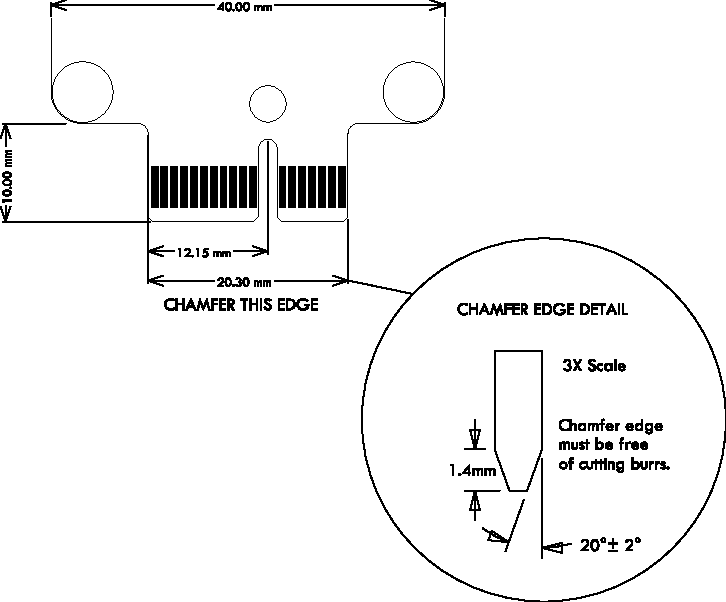
\includegraphics[width=0.700\linewidth]{slicecarddetail.pdf}
\end{sidecaption}\end{figure} \DocumentFooterFix


Note that for quick, low cost boards using low cost PCB manufacturing, the chamfer is not required and can be generated by hand using a file or similar.



% NON-FULLWIDTH SECTION
\section{Connector Pinouts}
\label{design_your_own:connector-pinouts}

The pinouts of the four types of sliceCARD are shown below. To cross reference pin numbers (eg. X0D1) to port names, see~here (see~\Sec~\ref{a16_core_board:sec-io-crossref}):



% NON-FULLWIDTH SECTION
\subsection{STAR}
\label{design_your_own:star}
\begin{tabular}{lll}
\Toprule
\textbf{PIN} & \textbf{SIDE B
(top)} & \textbf{SIDE A
(bottom)}\\
\midrule
1 & NC & NC\\
2 & NC & \emph{5V}\\
3 & \emph{GND} & NC\\
4 & NC & NC\\
5 & \emph{3V3} & \emph{GND}\\
6 & X0D2 & X0D8\\
7 & X0D3 & X0D9\\
8 & \emph{GND} & X0D1\\
9 & X0D4 & X0D6\\
10 & X0D10 & \emph{GND}\\
11 & X0D3 & X0D7\\
\multicolumn{3}{>{\setlength{\hsize}{3\hsize}\addtolength{\hsize}{3\tabcolsep}}l}{\textbf{MECHANICAL KEY}}\\
12 & X0D14 & X0D20\\
13 & X0D15 & X0D21\\
14 & \emph{CLK} & \emph{GND}\\
15 & X0D22 & X0D13\\
16 & \emph{GND} & \emph{RST\_N}\\
17 & X0D16 & X0D18\\
18 & X0D17 & X0D19\\
\bottomrule
\end{tabular}




% NON-FULLWIDTH SECTION
\subsection{SQUARE}
\label{design_your_own:square}
\begin{tabular}{lll}
\Toprule
\textbf{PIN} & \textbf{SIDE B
(top)} & \textbf{SIDE A
(bottom)}\\
\midrule
1 & \emph{DEBUG} & \emph{MSEL}\\
2 & \emph{TCK} & \emph{5V}\\
3 & \emph{GND} & \emph{TMS}\\
4 & \emph{TDI} & \emph{TDO}\\
5 & \emph{3V3} & \emph{PRSNT}\\
6 & X1D2 & X1D8\\
7 & X1D3 & X1D9\\
8 & \emph{GND} & X1D1\\
9 & X1D4 & X1D6\\
10 & X1D10 & \emph{GND}\\
11 & X1D3 & X1D7\\
\multicolumn{3}{>{\setlength{\hsize}{3\hsize}\addtolength{\hsize}{3\tabcolsep}}l}{\textbf{MECHANICAL KEY}}\\
12 & X1D14 & X1D20\\
13 & X1D15 & X1D21\\
14 & \emph{CLK} & \emph{GND}\\
15 & X1D22 & X1D13\\
16 & \emph{GND} & \emph{RST\_N}\\
17 & X1D16 & X1D18\\
18 & X1D17 & X1D19\\
\bottomrule
\end{tabular}




% NON-FULLWIDTH SECTION
\subsection{TRIANGLE}
\label{design_your_own:triangle}
\begin{tabular}{lll}
\Toprule
\textbf{PIN} & \textbf{SIDE B
(top)} & \textbf{SIDE A
(bottom)}\\
\midrule
1 & NC & NC\\
2 & X0D0 & \emph{5V}\\
3 & \emph{GND} & X0D12\\
4 & X0D11 & X0D23\\
5 & \emph{3V3} & \emph{GND}\\
6 & X0D26 & X0D32\\
7 & X0D27 & X0D33\\
8 & \emph{GND} & X0D25\\
9 & X0D28 & X0D30\\
10 & X0D34 & \emph{GND}\\
11 & X0D29 & X0D31\\
\multicolumn{3}{>{\setlength{\hsize}{3\hsize}\addtolength{\hsize}{3\tabcolsep}}l}{\textbf{MECHANICAL KEY}}\\
12 & X0D36 & X0D42\\
13 & X0D37 & X0D43\\
14 & \emph{CLK} & \emph{GND}\\
15 & X0D24 & X0D35\\
16 & \emph{GND} & \emph{RST\_N}\\
17 & X0D38 & X0D40\\
18 & X0D39 & X0D41\\
\bottomrule
\end{tabular}




% NON-FULLWIDTH SECTION
\subsection{CIRCLE}
\label{design_your_own:circle}
\begin{tabular}{lll}
\Toprule
\textbf{PIN} & \textbf{SIDE B
(top)} & \textbf{SIDE A
(bottom)}\\
\midrule
1 & NC & NC\\
2 & X1D0 & \emph{5V}\\
3 & \emph{GND} & X1D12\\
4 & X1D11 & X1D23\\
5 & \emph{3V3} & \emph{GND}\\
6 & X1D26 & X1D32\\
7 & X1D27 & X1D33\\
8 & \emph{GND} & X1D25\\
9 & X1D28 & X1D30\\
10 & X1D34 & \emph{GND}\\
11 & X1D29 & X1D31\\
\multicolumn{3}{>{\setlength{\hsize}{3\hsize}\addtolength{\hsize}{3\tabcolsep}}l}{\textbf{MECHANICAL KEY}}\\
12 & X1D36 & X1D42\\
13 & X1D37 & X1D43\\
14 & \emph{CLK} & \emph{GND}\\
15 & X1D24 & X1D35\\
16 & \emph{GND} & \emph{RST\_N}\\
17 & X1D38 & X1D40\\
18 & X1D39 & X1D41\\
\bottomrule
\end{tabular}




% NON-FULLWIDTH SECTION
\subsection{MIXED SIGNAL}
\label{design_your_own:mixed-signal}
\begin{tabular}{lll}
\Toprule
\textbf{PIN} & \textbf{SIDE B
(top)} & \textbf{SIDE A
(bottom)}\\
\midrule
1 & \emph{3V3A} & NC\\
2 & X0D10 & \emph{5V}\\
3 & \emph{GND} & X0D13\\
4 & X0D22 & WAKE\\
5 & \emph{3V3} & \emph{GND}\\
6 & ADC0 & ADC4\\
7 & ADC1 & ADC5\\
8 & \emph{GND} & \emph{GND}\\
9 & \emph{GND} & ADC6\\
10 & ADC2 & \emph{GND}\\
11 & ADC3 & \emph{GND}\\
\multicolumn{3}{>{\setlength{\hsize}{3\hsize}\addtolength{\hsize}{3\tabcolsep}}l}{\textbf{MECHANICAL KEY}}\\
12 & \emph{GND} & NC\\
13 & NC & NC\\
14 & NC & \emph{GND}\\
15 & X0D1 & NC\\
16 & \emph{GND} & \emph{RST\_N}\\
17 & \emph{GND} & ADC7\\
18 & NC & \emph{GND}\\
\bottomrule
\end{tabular}




\posttoc

\finish
